\documentclass[aspectratio=169,UTF8]{ctexbeamer}

\usefonttheme{professionalfonts}
\setbeamertemplate{navigation symbols}{}
\setbeamertemplate{footline}{
  \leavevmode
  \hbox{%
    \begin{beamercolorbox}[wd=.74\paperwidth,ht=2.4ex,dp=1ex,leftskip=1em]{footline}%
      DatawiseAgent 复现与改进
    \end{beamercolorbox}%
    \begin{beamercolorbox}[wd=.26\paperwidth,ht=2.4ex,dp=1ex,rightskip=1em plus 1fil]{footline}%
      \insertframenumber/\inserttotalframenumber
    \end{beamercolorbox}%
  }
}
\setbeamertemplate{frametitle}{
  \vspace{0.4em}
  \begin{beamercolorbox}[wd=\paperwidth,ht=3.2ex,dp=1.1ex,leftskip=1em]{frametitle}
    \insertframetitle
  \end{beamercolorbox}
}

\usepackage{booktabs}
\usepackage{tabularx}
\usepackage{array}
\usepackage{tikz}
\usetikzlibrary{positioning,arrows.meta,shapes.geometric}

\definecolor{DWBlue}{HTML}{244C8A}
\definecolor{DWLight}{HTML}{EEF4FB}
\definecolor{DWPale}{HTML}{F7F9FC}
\definecolor{DWGold}{HTML}{F2C94C}
\definecolor{DWGreen}{HTML}{2E7D32}
\definecolor{DWRed}{HTML}{B23A48}
\definecolor{DWGray}{HTML}{444444}

\setbeamercolor{background canvas}{bg=DWPale}
\setbeamercolor{frametitle}{fg=white,bg=DWBlue}
\setbeamercolor{footline}{fg=white,bg=DWBlue}
\setbeamercolor{block title}{fg=white,bg=DWBlue}
\setbeamercolor{block body}{fg=black,bg=white}
\setbeamercolor{alertblock title}{fg=white,bg=DWRed}
\setbeamercolor{alertblock body}{fg=black,bg=DWRed!8}
\setbeamercolor{takeaway}{fg=black,bg=DWGold!25}
\setbeamercolor{chip}{fg=DWBlue,bg=DWBlue!10}

\setbeamersize{text margin left=8mm,text margin right=8mm}
\setlength{\parskip}{0.25em}
\renewcommand{\arraystretch}{1.12}

\newcommand{\observed}{\textcolor{DWGreen}{Observed / 已观察}}
\newcommand{\diagnosed}{\textcolor{DWBlue}{Diagnosed / 已诊断}}
\newcommand{\planned}{\textcolor{DWRed}{Planned / 待验证}}
\newcommand{\hypothesis}{\textcolor{DWBlue}{hypothesis / target}}
\newcommand{\risk}{\textcolor{DWRed}{风险}}
\newcommand{\code}[1]{\texttt{\detokenize{#1}}}
\newcommand{\smallnote}[1]{{\scriptsize\textcolor{DWGray}{#1}}}
\newcommand{\chip}[1]{\begingroup\setlength{\fboxsep}{2pt}\colorbox{DWBlue!10}{\scriptsize\textcolor{DWBlue}{#1}}\endgroup}
\newcommand{\takeaway}[1]{%
  \vspace{0.35em}
  \begin{beamercolorbox}[wd=\textwidth,sep=0.75ex,rounded=true]{takeaway}
    \textbf{Takeaway：}#1
  \end{beamercolorbox}
}
\newcommand{\metric}[2]{%
  \begin{beamercolorbox}[wd=.92\linewidth,sep=0.8ex,rounded=true,center]{chip}
    {\Large\textbf{#1}}\\[-0.2em]{\scriptsize #2}
  \end{beamercolorbox}
}
\newcommand{\parttitle}[3]{%
  \begin{frame}[plain]
    \vspace{1.4em}
    \begin{center}
      \chip{#1}\\[1.0em]
      {\Huge\textbf{#2}}\\[0.7em]
      {\large #3}
    \end{center}
  \end{frame}
}

\title{从复现到改进：让 DatawiseAgent 的任务适配、长交互和资源预算可控}
\subtitle{InfiAgentBench / DataModeling 上的失败模式、结构化 harness 与资源感知调度}
\author{汇报人：於之翔，组员：冉子易 张恒}
\date{2026.6.10}

\begin{document}

\begin{frame}
  \vspace{1.0em}
  \begin{center}
    {\Huge\textbf{DatawiseAgent}}\\[0.5em]
    {\Large 复现改进：任务适配、长交互和资源预算可控}\\[4.2em]
    汇报人：於之翔，组员：冉子易、张恒\\[0.45em]
    2026.6.10
  \end{center}
\end{frame}

\begin{frame}{三条优化线}
\footnotesize
\begin{tabularx}{\textwidth}{p{0.20\textwidth} X}
\toprule
方向 & 核心问题 \\
\midrule
1. 任务适配 &
不同 benchmark 的失败源并不一致。InfiAgentBench 主要暴露答案名、统计口径、预处理顺序和最终格式不稳定；DataModeling 则更多暴露 submission 合法但预测低信息、metric 和 manifest 不完整等问题。因此 harness 不能只做统一 prompt，而要先识别任务类型和错误源。 \\
\midrule
2. 结构化时间换性能 &
长交互只有在每一轮都有明确检查目标时才有意义。我们需要把 planning、执行、debug、reformat 拆成可验证环节，失败时只修失败点，并用 final block / verifier 避免从长日志中漏抽或错抽答案。 \\
\midrule
3. 资源感知调度 &
强模型并不一定更慢，小模型也不一定更省。资源优化的核心是把确定性 schema、contract、format checker 前置，把强模型留给高风险推理和复杂代码生成，同时减少重复探索和无效对话。 \\
\bottomrule
\end{tabularx}
\takeaway{三条线不是堆模块：先识别任务错法，再把交互结构化，最后按风险决定模型、记忆和预算。}
\end{frame}

\parttitle{Part I}{Task-Specific Adaptation}{不同任务错法不同，harness 系统根据具体问题设计}

\begin{frame}{两个 Benchmark}
\footnotesize
\begin{columns}[T]
\begin{column}{0.49\textwidth}
\textbf{InfiAgentBench baseline / strong reference}
\vspace{0.3em}

\begin{tabularx}{\textwidth}{X r r r}
\toprule
Setting & ABQ & PASQ & UASQ \\
\midrule
Qwen3-32B full latest & 81.74\% & 86.21\% & 86.43\% \\
Qwen3.5-35B-A3B baseline & 86.38\% & 90.16\% & 90.35\% \\
\bottomrule
\end{tabularx}
\end{column}
\begin{column}{0.49\textwidth}
\textbf{DataModeling baseline / strong reference}
\vspace{0.3em}

\begin{tabularx}{\textwidth}{X r r r}
\toprule
Run & Complete & Perf. & Avg time \\
\midrule
qwen25 & 68/74 & 0.4290 & 760.25s \\
qwen35b-a3b-full & 73/74 & 0.5318 & 288.60s \\
\bottomrule
\end{tabularx}
\end{column}
\end{columns}
\vspace{0.7em}
\begin{alertblock}{共同结论}
通过强模型，了解答案正确率上限，同时也说明好的理解和规划可以在正确率及耗时上获得高效提升。我们的优化目标就是通过整合系统、记忆等 harness 技巧，让弱模型也能实现强模型的正确率。但针对不同任务，我们需要分别分析他们的错误源。
\end{alertblock}
\end{frame}

<<<<<<< HEAD:docs/report_beamer.tex
\begin{frame}{口径漂移}
\small
\begin{columns}[T]
\begin{column}{0.42\textwidth}
\begin{alertblock}{核心问题}
\Large\textbf{代码能跑，\newline 但答案口径不稳定}
\vspace{0.55em}

\normalsize
同一张表、同一个问题，模型可能在过滤条件、统计方法、小数位或最终格式上发生轻微漂移；这些错误不一定报错，但会直接影响闭式评分。
\end{alertblock}
\end{column}
\begin{column}{0.55\textwidth}
\begin{block}{Task-Aware harness}
\begin{enumerate}
  \item 先用 \textbf{level / concepts / keywords / format} 识别题型；
  \item 不同题型路由到对应 \textbf{Harness Protocol}；
  \item protocol 约束执行，并要求可复现证据；
  \item verifier 检查输出是否符合任务契约。
\end{enumerate}
\end{block}
\end{column}
\end{columns}
\vspace{0.45em}
\begin{center}
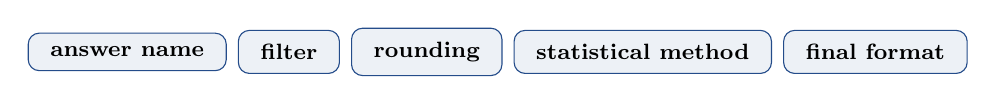
\begin{tikzpicture}[node distance=0.14cm]
  \node[draw=DWBlue, fill=DWBlue!8, rounded corners, inner xsep=8pt, inner ysep=5pt, font=\footnotesize\bfseries] (a) {answer name};
  \node[draw=DWBlue, fill=DWBlue!8, rounded corners, inner xsep=8pt, inner ysep=5pt, font=\footnotesize\bfseries, right=of a] (b) {filter};
  \node[draw=DWBlue, fill=DWBlue!8, rounded corners, inner xsep=8pt, inner ysep=5pt, font=\footnotesize\bfseries, right=of b] (c) {rounding};
  \node[draw=DWBlue, fill=DWBlue!8, rounded corners, inner xsep=8pt, inner ysep=5pt, font=\footnotesize\bfseries, right=of c] (d) {statistical method};
  \node[draw=DWBlue, fill=DWBlue!8, rounded corners, inner xsep=8pt, inner ysep=5pt, font=\footnotesize\bfseries, right=of d] (e) {final format};
\end{tikzpicture}
\end{center}
\takeaway{重点不是让模型“知道答案”，而是把题目口径显式化为 execution contract：任务决定协议，协议约束执行，验证决定能否输出。}
\end{frame}


\begin{frame}{Task Router}
\footnotesize
\begin{columns}[T]
\begin{column}{0.34\textwidth}
\begin{block}{路由信号}
=======
\begin{frame}{Part I Ananlysis：InfiAgentBench 格式约束不足}
\begin{columns}[T]
\begin{column}{0.49\textwidth}
\begin{block}{常见失败}
>>>>>>> parent of 9d26969 (Refine Beamer task-aware harness narrative):docs/expected_results_beamer.tex
\begin{itemize}
  \item 最终答案格式、小数位、引号、dict/list 格式错误；
  \item 预处理顺序、子集口径、缺失值处理错误；
  \item 相关性、显著性、正态性、异常值判断错误；
  \item 特征工程公式理解错误；
  \item reformat 从长日志中漏抽、错抽。
\end{itemize}
\end{block}
\end{column}
\begin{column}{0.48\textwidth}
\begin{alertblock}{关键判断}
很多题不是“代码完全不会写”，而是：
\begin{itemize}
  \item 题目约束没有提前固定；
  \item 统计语义没有过程校验；
  \item 最终答案通道不稳定。
\end{itemize}
\end{alertblock}
\end{column}
\end{columns}
\takeaway{InfiAgentBench 需要 answer-aware harness：从答案名、口径、统计方法和最终格式这些方面中设计约束。}
\end{frame}

\begin{frame}{Part I Scheme：InfiAgentBench answer-aware harness}
\footnotesize
\begin{tabularx}{\textwidth}{p{0.20\textwidth} X p{0.27\textwidth}}
\toprule
模块 & 作用 & 对应错误 \\
\midrule
DataCard & 固定 CSV 结构，记录列名、dtype、缺失值、范围、类别样例。 & 列选择、缺失值、类型误判 \\
Contract & 抽取 answer name、列、过滤条件、操作、小数位、输出容器。 & 口径、格式、额外清洗 \\
Skill checklist & 针对 correlation、outlier、ML、format 等题型给检查清单。 & 统计方法、ML 协议 \\
Verifier & 检查列、样本数、p-value、abs(r)、split、final block。 & 代码能跑但语义错 \\
Final Block & 机器可读答案块，再确定性转 \code{@answer[value]}。 & reformat 漏抽、占位符 \\
\bottomrule
\end{tabularx}
\end{frame}

\begin{frame}{DataModeling Protocol}
\small
\begin{columns}[T]
\begin{column}{0.49\textwidth}
\begin{block}{基于 InfiAgentBench 已有的改动}
\begin{itemize}
  \item Contract / Profile：固定 metric、列、行数、target；
  \item Task Router：tabular、text、time-series、multi-output；
  \item Submission Validator：schema、ID、概率范围、sample copy；
  \item Quality Gate：manifest、fallback、常数预测、低信息 final。
\end{itemize}
\end{block}
\end{column}
\begin{column}{0.49\textwidth}
\begin{alertblock}{依旧存在的问题}
\begin{itemize}
  \item 结构合法但只是 fallback；
  \item 多分类塌缩成单类；
  \item 回归/概率输出全局均值；
  \item CSV 可评，但没有 validation 和选择依据。
\end{itemize}
\end{alertblock}
\end{column}
\end{columns}
\takeaway{这一步不替模型建模，只把提交前能检查清楚的内容先检查清楚。}
\end{frame}

<<<<<<< HEAD:docs/report_beamer.tex
\begin{frame}{Harness 收益}
=======
\begin{frame}{Part I Result：InfiAgentBench harness 结果}
>>>>>>> parent of 9d26969 (Refine Beamer task-aware harness narrative):docs/expected_results_beamer.tex
\footnotesize
\begin{tabularx}{\textwidth}{p{0.34\textwidth} p{0.14\textwidth} r r r}
\toprule
Setting & Split & ABQ & PASQ & UASQ \\
\midrule
Qwen3-32B baseline & medium & 83.72\% & 86.19\% & 86.00\% \\
Harness rerender & medium & 91.95\% & 93.06\% & 93.42\% \\
\midrule
Qwen3-32B baseline & hard & 66.13\% & 78.49\% & 82.99\% \\
Harness rerender & hard & 78.41\% & 84.75\% & 87.19\% \\
\bottomrule
\end{tabularx}
\vspace{0.65em}
\begin{columns}[T]
\begin{column}{0.32\textwidth}
\begin{block}{medium}
ABQ 提升 8.23 个百分点，说明格式约束和结果抽取能直接减少可避免错误。
\end{block}
\end{column}
\begin{column}{0.32\textwidth}
\begin{block}{hard}
ABQ 提升 12.28 个百分点，但平均分支数升至 2.97，复杂题仍需要控制搜索成本。
\end{block}
\end{column}
\begin{column}{0.32\textwidth}
\begin{block}{答案通道}
format error、reformat missing、final block missing 均为 0，说明结构化答案链路有效。
\end{block}
\end{column}
\end{columns}
\end{frame}

\begin{frame}{DataModeling 结果}
\footnotesize
\begin{tabularx}{\textwidth}{p{0.37\textwidth} r r r}
\toprule
Setting & Complete & Perf. & Avg time \\
\midrule
qwen25 baseline & 68/74 & 0.4290 & 760.25s \\
qwen35b-a3b-full & 73/74 & 0.5318 & 288.60s \\
qwen3-vl-8b old harness & 74/74 & 0.3127 & 799.09s \\
qwen3-vl-32b old harness & 74/74 & 0.2873 & 297.49s \\
\bottomrule
\end{tabularx}
\vspace{0.65em}
\begin{columns}[T]
\begin{column}{0.33\textwidth}\metric{+0.1028}{qwen35b vs qwen25}\end{column}
\begin{column}{0.33\textwidth}\metric{74/74}{qwen3-vl completion}\end{column}
\begin{column}{0.33\textwidth}\metric{0.45--0.50}{修复典型模式后的目标区间}\end{column}
\end{columns}
\vspace{0.45em}
\smallnote{qwen3-vl 的问题不是不能交文件，而是合法 CSV 里常有均值、常数、fallback 或 manifest 缺失。}
\takeaway{DataModeling 已经证明强模型与工程约束有收益；弱模型暴露的是 completion 到 performance 的关键断点。}
\end{frame}

\begin{frame}{难度分层}
\footnotesize
\begin{columns}[T]
\begin{column}{0.32\textwidth}
\begin{block}{有逻辑可循的任务}
Titanic、Santander 这类 schema / metric 清晰的 tabular 任务，contract 与 validator 能帮助模型走到有效路径。
\end{block}
\end{column}
\begin{column}{0.32\textwidth}
\begin{block}{低分集中模式}
多分类塌缩、均值回归、文本错路由、多输出常数、时间/分组任务错当普通表格。
\end{block}
\end{column}
\begin{column}{0.32\textwidth}
\begin{alertblock}{下一步}
manifest-only repair、分级 early-stop、任务族模板、低信息预测拦截。
\end{alertblock}
\end{column}
\end{columns}
\vspace{0.25em}
\begin{tabularx}{\textwidth}{p{0.30\textwidth} r X}
\toprule
代表复测 & 分数 & 说明 \\
\midrule
8B Titanic & 0.7877 & 有效 tabular submission；manifest 需要短修复 \\
32B Titanic & 0.7709 & 大模型不自动更好，仍受流程厚度影响 \\
32B Santander & 0.8116 & 预测质量可用，耗时和 manifest 是主要瓶颈 \\
\bottomrule
\end{tabularx}
\takeaway{弱模型低分帮助定位：哪些题需轻约束，哪些题必须进入质量驱动流程。}
\end{frame}

\begin{frame}{负结果}
\footnotesize
\begin{columns}[T]
\begin{column}{0.32\textwidth}
\begin{block}{1. Harness 要适配模型}
弱模型不能配过厚、过死的流程；目标是按风险调度，而不是 full-everywhere。
\end{block}
\end{column}
\begin{column}{0.32\textwidth}
\begin{block}{2. 记忆不能全记住}
旧记忆、低价值记忆会降低信噪比；记忆系统需要重要性、时效性和遗忘机制。
\end{block}
\end{column}
\begin{column}{0.32\textwidth}
\begin{block}{3. Training-free 有上限}
DataModeling 跨任务难度大；工程能改路径和验证，但不能完全替代强模型或后训练。
\end{block}
\end{column}
\end{columns}
\vspace{-0.2em}
\begin{center}
\begin{tikzpicture}[x=1cm,y=0.82cm]
  \draw[->, thick, DWGray] (0,0) -- (8.6,0) node[right, font=\scriptsize]{memory 时间};
  \draw[->, thick, DWGray] (0,0) -- (0,2.05) node[above, font=\scriptsize]{广义成本};
  \draw[very thick, DWRed] plot[smooth] coordinates {(0.2,0.25) (2,0.55) (4,1.05) (6,1.65) (8.1,2.05)};
  \draw[very thick, DWGreen] plot[smooth] coordinates {(0.2,0.28) (2,0.52) (4,0.65) (6,0.70) (8.1,0.73)};
  \node[DWRed, font=\scriptsize] at (6.8,1.74) {全记住：噪声和上下文压力上升};
  \node[DWGreen, font=\scriptsize] at (6.45,0.46) {可控遗忘：检索质量稳定};
\end{tikzpicture}
\end{center}
\takeaway{失败 insight 把边界讲清楚：模型能力、记忆质量和 harness 厚度必须一起调。}
\end{frame}

\parttitle{Part II}{Weak Model + Harness}{不是多问几轮，而是把多出来的时间花在检查上}

\begin{frame}{实验口径}
\scriptsize
\renewcommand{\arraystretch}{1.08}
\begin{tabularx}{\textwidth}{p{0.22\textwidth} X X}
\toprule
Setting & 操作 & 意义 \\
\midrule
baseline + reformat &
qwen3.5-flash 按原始 DatawiseAgent 流程输出长日志，再走原始 reformat 抽取闭式答案。 &
弱模型原始能力 + 原始答案抽取。 \\
\midrule
\code{harness_light} &
轻量检查版：DataCard、题目要求、基础检查清单、Final Block 收束；关闭 search、memory、heavy oracle / verifier。 &
目标是先修低级但致命的错：列名、格式、小数位、答案名和最终输出通道。 \\
\midrule
\code{harness_full} &
重检查版：加入更多中间结果检查、候选检查和失败处理。 &
目标是继续提分，但代价是更慢；检查太严时也可能阻断可解析答案。 \\
\bottomrule
\end{tabularx}
\renewcommand{\arraystretch}{1.0}
\end{frame}

\begin{frame}{全集结果}
\footnotesize
\begin{tabularx}{\textwidth}{p{0.31\textwidth} r r r}
\toprule
Setting & ABQ & Hard ABQ & Avg runtime \\
\midrule
baseline + original reformat & 48.94\% & 44.00\% & 30.24s \\
\code{harness_light} & 59.57\% & 60.00\% & 47.03s \\
\code{harness_full} & 63.83\% & 64.00\% & 92.79s \\
\bottomrule
\end{tabularx}
\vspace{0.65em}
\begin{columns}[T]
\begin{column}{0.31\textwidth}
\metric{+10.63}{light vs baseline ABQ}
\end{column}
\begin{column}{0.31\textwidth}
\metric{+16.00}{light vs baseline hard ABQ}
\end{column}
\begin{column}{0.31\textwidth}
\metric{+16.79s}{light runtime 增量}
\end{column}
\end{columns}
\vspace{0.45em}
\begin{alertblock}{趋势}
47 道 small error set + full 257 和完整消融已验证，弱模型在部分效果是有接近强模型的趋势。
\end{alertblock}
\takeaway{light 提分明显，额外时间还能接受；full 分数最高，但 runtime 变得很重。}
\end{frame}

\begin{frame}{实验意义}
\footnotesize
\begin{columns}[T]
\begin{column}{0.50\textwidth}
\begin{block}{弱模型主要不是“完全不会”}
\begin{itemize}
  \item 会写代码，但容易漏题目要求；
  \item 会算结果，但小数位、答案名、容器格式不稳；
  \item 会跑统计，但可能漏筛选条件或比较口径。
\end{itemize}
\end{block}
\end{column}
\begin{column}{0.46\textwidth}
\begin{alertblock}{检查带来的收益和代价}
\begin{itemize}
  \item light 修了很多低级但致命的错；
  \item full 还能再修一点，但时间成本上升；
  \item 所以不是越重越好，而是看题目风险。
\end{itemize}
\end{alertblock}
\end{column}
\end{columns}
\vspace{0.35em}
\scriptsize
\begin{tabularx}{\textwidth}{p{0.22\textwidth} X X}
\toprule
常见错法 & 轻量检查能做什么 & 重检查什么时候再上 \\
\midrule
格式 / 答案名错 & 用 Final Block 和程序化 reformat 收束。 & final block 缺失或格式不合法时。 \\
\midrule
列名 / 筛选漏掉 & 先给 DataCard 和题目要求列表。 & 中间结果样本数异常时。 \\
\midrule
统计口径不稳 & 给相关性、异常值、预处理顺序检查清单。 & hard 题、分支结果冲突或多次失败时。 \\
\bottomrule
\end{tabularx}
\takeaway{这个结果的价值是说明：弱模型的额外时间如果花在检查上，比单纯多问几轮更有效。}
\end{frame}

\begin{frame}{时间花在哪}
\footnotesize
\begin{center}
\resizebox{\textwidth}{!}{%
\begin{tikzpicture}[
  node distance=0.55cm and 0.40cm,
  box/.style={draw=DWBlue, fill=white, rounded corners, align=center, minimum width=1.9cm, minimum height=0.72cm, font=\scriptsize},
  emph/.style={draw=DWBlue, fill=DWBlue!9, rounded corners, align=center, minimum width=1.9cm, minimum height=0.72cm, font=\scriptsize\bfseries},
  arrow/.style={-{Latex[length=2mm]}, thick, draw=DWBlue}
]
\node[emph] (q) {Question\\+ CSV};
\node[box, right=of q] (data) {DataCard\\列名/缺失};
\node[box, right=of data] (req) {题目要求\\答案格式};
\node[box, right=of req] (skill) {检查清单\\统计/格式};
\node[box, right=of skill] (exec) {Notebook\\执行};
\node[box, right=of exec] (check) {中间结果\\检查};
\node[emph, right=of check] (final) {Final Block\\程序化输出};
\draw[arrow] (q) -- (data);
\draw[arrow] (data) -- (req);
\draw[arrow] (req) -- (skill);
\draw[arrow] (skill) -- (exec);
\draw[arrow] (exec) -- (check);
\draw[arrow] (check) -- (final);
\draw[arrow, dashed] (check.south) to[out=-80,in=-100] node[below, font=\scriptsize, text=DWRed]{检查不过才短修复} (exec.south);
\end{tikzpicture}
}
\end{center}
\vspace{0.45em}
\begin{columns}[T]
\begin{column}{0.48\textwidth}
\begin{block}{程序能直接判断的}
\begin{itemize}
  \item 列是否存在，筛选后是否为空；
  \item final block 是否是合法 JSON；
  \item 小数位、列表 / 字典、\code{@answer} 是否匹配。
\end{itemize}
\end{block}
\end{column}
\begin{column}{0.48\textwidth}
\begin{alertblock}{模型还需要判断的}
\begin{itemize}
  \item 题目到底要哪个统计口径；
  \item 多个候选结果哪个更可信；
  \item 检查失败后应修代码还是修答案。
\end{itemize}
\end{alertblock}
\end{column}
\end{columns}
\takeaway{关键不是把所有事都交给模型，而是能程序检查的先程序检查，复杂判断再交给模型。}
\end{frame}

\begin{frame}{过渡}
\footnotesize
\begin{columns}[T]
\begin{column}{0.50\textwidth}
\begin{block}{从 small set 得到的结论}
\begin{itemize}
  \item 弱模型加轻量检查能明显提分；
  \item 重检查继续提分，但 runtime 从 47.03s 到 92.79s；
  \item 所以下一步不是继续加模块，而是判断什么时候值得多花时间。
\end{itemize}
\end{block}
\end{column}
\begin{column}{0.46\textwidth}
\begin{alertblock}{第三部分要回答}
\begin{itemize}
  \item 简单步骤能不能规则化？
  \item 明确子任务能不能交给小模型？
  \item 复杂规划、候选选择、失败兜底何时上强 thinking 模型？
  \item sub-agent 通信会不会抵消收益？
\end{itemize}
\end{alertblock}
\end{column}
\end{columns}
\vspace{0.4em}
\begin{center}
\resizebox{0.88\textwidth}{!}{%
\begin{tikzpicture}[
  node distance=0.70cm,
  box/.style={draw=DWBlue, fill=white, rounded corners, align=center, minimum width=2.35cm, minimum height=0.72cm, font=\scriptsize},
  arrow/.style={-{Latex[length=2mm]}, thick, draw=DWBlue}
]
\node[box] (a) {light-first\\先少折腾};
\node[box, right=of a] (b) {检查不过\\短修复};
\node[box, right=of b] (c) {高风险\\强模型兜底};
\node[box, right=of c] (d) {记录成本\\EqTok/runtime};
\draw[arrow] (a) -- (b);
\draw[arrow] (b) -- (c);
\draw[arrow] (c) -- (d);
\end{tikzpicture}
}
\end{center}
\takeaway{Part II 讲清楚“时间花在哪里”；Part III 继续讨论“由谁来花、哪些调用可以省”。}
\end{frame}

\parttitle{Part III}{Resource-Aware Plan}{把时间分给合适的模型；能不问模型就不问}

\begin{frame}{方案边界}
\footnotesize
\begin{columns}[T]
\begin{column}{0.46\textwidth}
\begin{block}{先说边界}
\begin{itemize}
  \item resource-aware / sub-agent 还没完整验证；
  \item 这里主要讲后续实验设计；
  \item 指标用 EqTok、调用次数、runtime 一起看。
\end{itemize}
\end{block}
\end{column}
\begin{column}{0.52\textwidth}
\begin{alertblock}{等效 token}
\[
\mathrm{EqTok}=T_{32B}+0.5T_{14B}+0.25T_{8B}
\]
\footnotesize
把 32B / 14B / 8B 的消耗放到同一把尺上；路由收益仍是 expected / 待验证。
\end{alertblock}
\end{column}
\end{columns}
\vspace{0.15em}
\scriptsize
\renewcommand{\arraystretch}{1.04}
\begin{tabularx}{\textwidth}{p{0.32\textwidth} r r r}
\toprule
参考线 / 预期项 & ABQ & EqTok & 状态 \\
\midrule
Qwen3-32B full baseline & 81.74\% & 5.961M & 参考线 \\
小模型路由 & 80.5--82.5\% & 约 2.120M & expected \\
路由 + 减少对话 & 81.0--83.5\% & 1.05--1.60M & target / 待验证 \\
\bottomrule
\end{tabularx}
\renewcommand{\arraystretch}{1.0}
\takeaway{这页不是说已经省下成本，而是给后续实验一个清楚的资源账本。}
\end{frame}

\begin{frame}{两个抓手}
\scriptsize
\renewcommand{\arraystretch}{1.04}
\begin{tabularx}{\textwidth}{p{0.24\textwidth} X X}
\toprule
抓手 & 做法 & 答辩时怎么解释 \\
\midrule
换小模型 / 规则 & 固定数据检查、答案格式、列名匹配、final answer 渲染尽量程序化；普通统计题走弱模型 + light。 & 输入短、标准明确，不需要强模型全流程参与。 \\
\midrule
直接省掉调用 & 同一 CSV 的 DataCard 复用；低风险题不反复 planning；检查通过就不再回传完整日志。 & 省掉重复确认和长日志回传，不省必要推理。 \\
\midrule
失败后再升级 & 多次检查不过、候选冲突、复杂统计口径不确定时，再交给强 thinking 模型。 & 32B-thinking 可以做主 Agent，但全流程使用成本高。 \\
\bottomrule
\end{tabularx}
\renewcommand{\arraystretch}{1.0}
\vspace{0.25em}
\begin{alertblock}{一句话回答 planning 问题}
planning 仍然重要；我们只是把 schema、格式渲染、列名检查、固定统计这类不需要重新规划的步骤拿出来，减少无意义 planning 调用。
\end{alertblock}
\takeaway{总方案不是“换成小模型”，而是少让大模型做无必要的事。}
\end{frame}

\begin{frame}{执行路径}
\footnotesize
\begin{center}
\resizebox{\textwidth}{!}{%
\begin{tikzpicture}[
  node distance=0.70cm and 0.48cm,
  box/.style={draw=DWBlue, fill=white, rounded corners, align=center, minimum width=2.0cm, minimum height=0.70cm, font=\scriptsize},
  emph/.style={draw=DWBlue, fill=DWBlue!9, rounded corners, align=center, minimum width=2.0cm, minimum height=0.70cm, font=\scriptsize\bfseries},
  arrow/.style={-{Latex[length=2mm]}, thick, draw=DWBlue}
]
\node[emph] (rule) {规则检查\\schema/format};
\node[box, right=of rule] (weak) {弱模型 + light\\普通统计题};
\node[box, right=of weak] (gate) {检查门\\通过?};
\node[box, right=of gate] (strong) {强模型\\复杂/兜底};
\node[emph, right=of strong] (final) {程序化\\final answer};
\draw[arrow] (rule) -- (weak);
\draw[arrow] (weak) -- (gate);
\draw[arrow] (gate) -- node[above, font=\scriptsize]{不过 / 高风险} (strong);
\draw[arrow] (strong) -- (final);
\draw[arrow, bend right=22] (gate.south) to node[below, font=\scriptsize]{通过} (final.south);
\end{tikzpicture}
}
\end{center}
\vspace{0.45em}
\begin{columns}[T]
\begin{column}{0.32\textwidth}
\begin{block}{强模型用在哪}
复杂规划、候选选择、失败兜底；不是所有格式和固定检查都交给它。
\end{block}
\end{column}
\begin{column}{0.32\textwidth}
\begin{block}{sub-agent 怎么拆}
只拆短、局部、结构化任务；否则通信轮次会抵消收益。
\end{block}
\end{column}
\begin{column}{0.32\textwidth}
\begin{block}{怎么验证}
记录 EqTok、调用次数、runtime、ABQ；先小集，再 full 257。
\end{block}
\end{column}
\end{columns}
\takeaway{第三部分的重点是后续实验路线：简单题少折腾，难题再多花时间。}
\end{frame}

\begin{frame}{待验证实验}
\scriptsize
\renewcommand{\arraystretch}{1.05}
\begin{tabularx}{\textwidth}{p{0.25\textwidth} X X}
\toprule
实验 & 要回答的问题 & 状态 \\
\midrule
full 257 baseline vs \code{harness_light} & small set 提升是否能外推到全量。 & 待验证 \\
\midrule
最小消融 & final block、检查清单、重检查分别贡献多少。 & 待验证 \\
\midrule
EqTok token meter & 成本是否真的下降，还是只把调用拆碎。 & 待实现 / 待验证 \\
\midrule
model routing & 什么时候用弱模型，什么时候强模型兜底。 & 后续方案 \\
\bottomrule
\end{tabularx}
\renewcommand{\arraystretch}{1.0}
\vspace{0.25em}
\begin{alertblock}{不要说满}
resource-aware、sub-agent、full 257、完整消融目前都不能当已完成结论；最多作为下一步路线和预期目标。
\end{alertblock}
\takeaway{第三部分最稳的讲法：我们已经看到检查能提分，下一步要证明怎么少花冤枉钱。}
\end{frame}

\parttitle{Takeaway}{What We Can Safely Claim}{已经看到的现象 + 下一步要补的实验}

\begin{frame}{结论边界}
\small
\begin{columns}[T]
\begin{column}{0.48\textwidth}
\begin{block}{能说的}
\begin{itemize}
  \item InfiAgentBench 错题小集上，light harness 明显提升；
  \item full 版本分数更高，但时间成本也明显更高；
  \item DataModeling 初步看，协议错误比单纯模型能力更突出。
\end{itemize}
\end{block}
\end{column}
\begin{column}{0.48\textwidth}
\begin{alertblock}{不能说满的}
\begin{itemize}
  \item full 257 还没有系统结论；
  \item resource-aware 和 sub-agent 还没有完整实验；
  \item DataModeling 还只是 protocol-aware 的动机，不是稳定提分验证。
\end{itemize}
\end{alertblock}
\end{column}
\end{columns}
\takeaway{当前最稳的结论是：轻量检查能帮助弱模型，但继续加重检查必须看时间成本和失败风险。}
\end{frame}

\begin{frame}{下一步}
\small
\begin{columns}[T]
\begin{column}{0.48\textwidth}
\begin{block}{实验优先级}
\begin{enumerate}
  \item qwen3.5-flash full 257：baseline vs light；
  \item 最小消融：no finalizer / no skills / no heavy check；
  \item 加 token meter：EqTok、调用次数、runtime；
  \item 再做 model routing / fallback。
\end{enumerate}
\end{block}
\end{column}
\begin{column}{0.48\textwidth}
\begin{alertblock}{汇报主线}
\begin{itemize}
  \item 简单题少折腾；
  \item 中等题用弱模型 + light 检查；
  \item 难题、失败题再多花时间；
  \item 强模型保留给复杂规划、候选选择和兜底。
\end{itemize}
\end{alertblock}
\end{column}
\end{columns}
\takeaway{我们不是说已经完成一个最优系统，而是把“长交互为什么有用”拆成了可以继续验证的实验问题。}
\end{frame}

\begin{frame}
\vspace{2.4em}
\begin{center}
{\Huge\textbf{感谢聆听}}
\end{center}
\end{frame}

\end{document}
